\documentclass[12pt]{article} % font size 12pt
\usepackage[a4paper, margin=20mm]{geometry} % a4 paper size, 20 mm margin
\usepackage{graphicx} % Required for inserting images
\usepackage{listings}
\usepackage{float}
\usepackage{amsmath}

\lstset{
  language=Python,
  basicstyle=\ttfamily\small,
  frame=single,
  breaklines=true
}

\title{Signal and Image Processing\\
Individual Assignment -- Week 4}
\author{Noah Junge: qxk266}
\date{January 2026}

\begin{document}

\maketitle

\section{Image Filtering}

\subsection{}
\textbf{Derive filter kernels for the approximate partial derivatives $\partial I / \partial x$ and $\partial I / \partial y$ using correlation. Show how the kernels differ when using convolution. Explain the center pixel position and why correlation vs convolution does not matter for Gaussian and mean filters.}

A finite difference approximation of the horizontal derivative at pixel $(x, y)$ is

$$\frac{\partial I}{\partial x}(x,y) \approx \frac{I(x+1,y) - I(x-1,y)}{2}$$

Expressed as a correlation $(I \star h)(x,y) = \sum_k h(k)\, I(x+k,\, y)$, this gives the kernels

$$h_x^{\text{corr}} = \begin{bmatrix} -1 & 0 & 1 \end{bmatrix}, \qquad h_y^{\text{corr}} = \begin{bmatrix} -1 \\ 0 \\ 1 \end{bmatrix}$$

\textbf{Center pixel.} The kernel has 3 elements with indices $k \in \{-1, 0, 1\}$, so the center element at $k = 0$ aligns the output with the pixel being differentiated.

\textbf{Convolution kernels.} Convolution flips the kernel: $(I * h)(x,y) = \sum_k h(k)\, I(x-k,\, y)$, giving

$$h_x^{\text{conv}} = \begin{bmatrix} 1 & 0 & -1 \end{bmatrix}, \qquad h_y^{\text{conv}} = \begin{bmatrix} 1 \\ 0 \\ -1 \end{bmatrix}$$

\textbf{Symmetric filters.} Both the Gaussian and mean kernels satisfy $h(k) = h(-k)$. Flipping a symmetric kernel yields the same kernel, so correlation and convolution produce identical results.

\subsection{}
\textbf{Write the $y$-derivative versions of the Prewitt and Sobel filters in separable form. Explain why they are more robust to noise than simple finite differences.}

The Prewitt filter smooths along one axis (uniform average) before differentiating along the other:

$$P_x = \begin{bmatrix}1\\1\\1\end{bmatrix} * \begin{bmatrix}-1 & 0 & 1\end{bmatrix}, \qquad P_y = \begin{bmatrix}-1\\0\\1\end{bmatrix} * \begin{bmatrix}1 & 1 & 1\end{bmatrix}$$

The Sobel filter uses a weighted average ($1\!:\!2\!:\!1$) instead:

$$S_x = \begin{bmatrix}1\\2\\1\end{bmatrix} * \begin{bmatrix}-1 & 0 & 1\end{bmatrix}, \qquad S_y = \begin{bmatrix}-1\\0\\1\end{bmatrix} * \begin{bmatrix}1 & 2 & 1\end{bmatrix}$$

\textbf{Noise robustness.} A simple finite difference $[-1\; 0\; 1]$ uses only two pixels, so noise in either pixel propagates directly into the derivative estimate. Prewitt and Sobel first average over three neighbouring rows or columns before differentiating, suppressing high-frequency noise while preserving the edge signal. The Sobel filter's $1\!:\!2\!:\!1$ weighting approximates a Gaussian pre-filter, giving slightly better noise reduction than Prewitt's uniform average.

\section{Segmentation by Thresholding}

\subsection{}
\textbf{Load \texttt{pillsect.png}, convert to grayscale, apply a threshold of 100, and show the original, grayscale, and binary images side by side.}

\begin{lstlisting}
img_pil = Image.open("pillsect.png")
gray = np.array(img_pil.convert("L"))

THRESHOLD = 100
binary = (gray > THRESHOLD).astype(np.uint8) * 255

fig, axes = plt.subplots(1, 3, figsize=(12, 4))
axes[0].imshow(np.array(img_pil));  axes[0].set_title("Original")
axes[1].imshow(gray, cmap="gray");  axes[1].set_title("Grayscale")
axes[2].imshow(binary, cmap="gray"); axes[2].set_title("Binary (threshold=100)")
\end{lstlisting}

\begin{figure}[H]
    \centering
    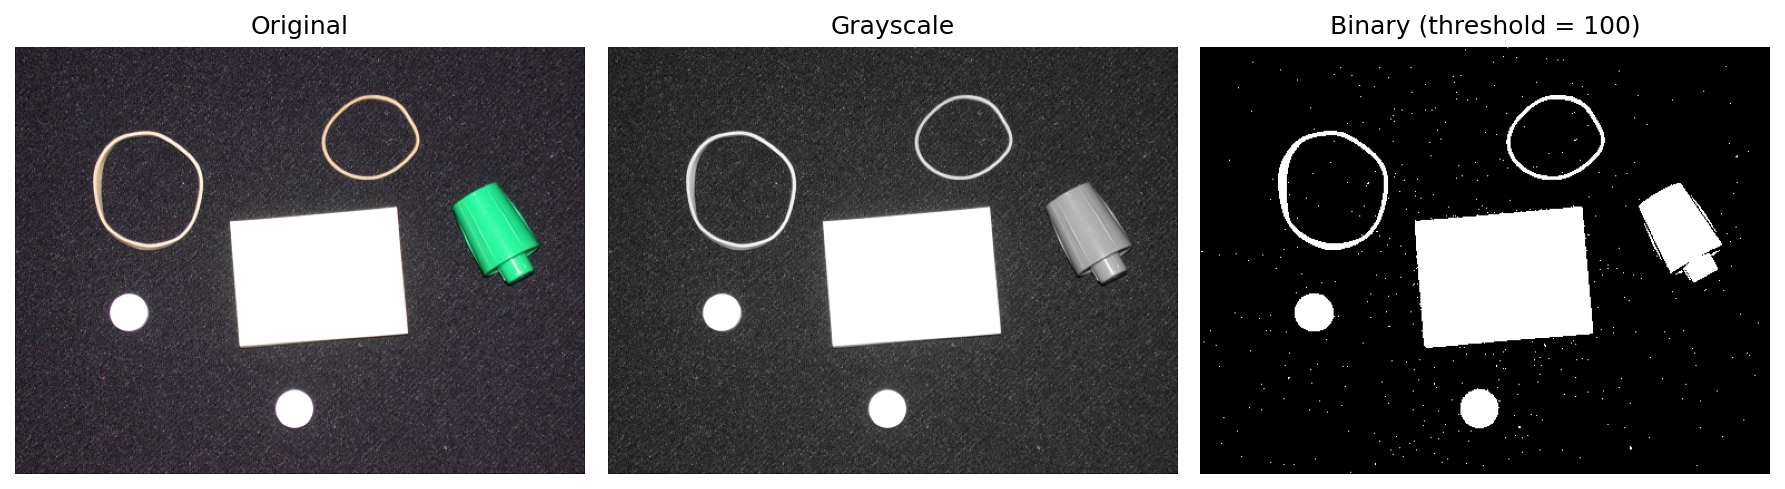
\includegraphics[width=\textwidth]{segmentation.png}
    \caption{Original, grayscale, and binary segmentation of \texttt{pillsect.png} at threshold $= 100$.}
\end{figure}

The dark background has intensities well below 100 and maps to black. All foreground objects (rings, rectangle, dots, cylinder) have intensities above 100 and map to white. The segmentation cleanly separates background from foreground, suggesting the threshold is well chosen.

\subsection{}
\textbf{Plot the intensity histogram and discuss the choice of threshold.}

\begin{figure}[H]
    \centering
    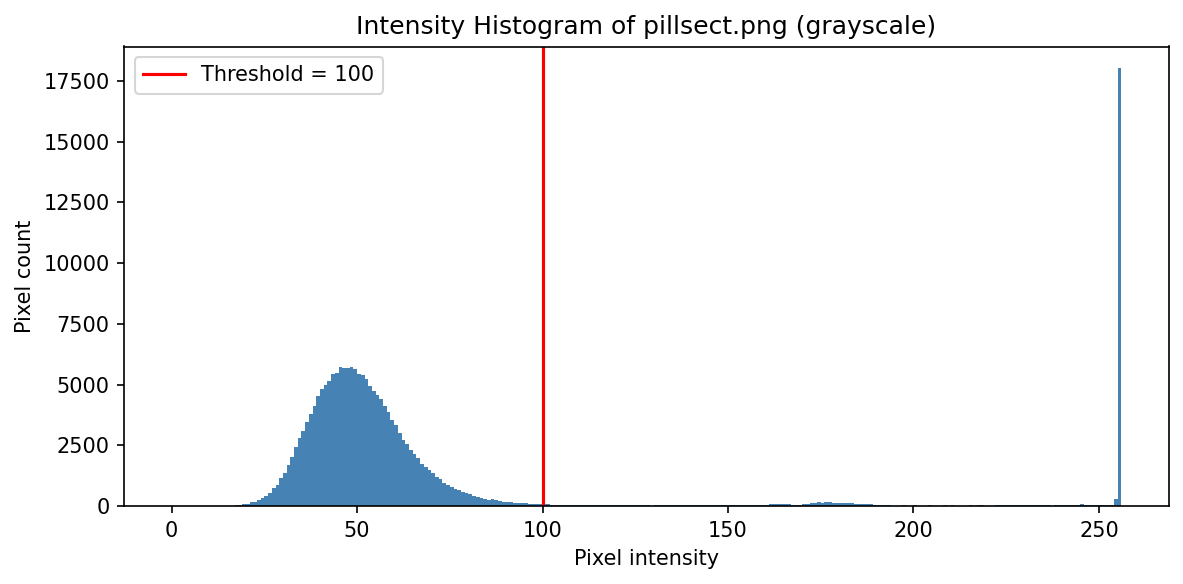
\includegraphics[width=0.8\textwidth]{histogram.png}
    \caption{Intensity histogram of the grayscale \texttt{pillsect.png}. The red line marks the threshold at 100.}
\end{figure}

The histogram shows a clear bimodal distribution: a large peak near intensity 0--30 from the dark background and a broader spread at higher intensities from the bright foreground objects. The threshold of 100 sits in the valley between the two peaks, making it an appropriate choice.

\begin{itemize}
    \item \textbf{Threshold too low (e.g.\ $< 50$):} Background pixels get classified as foreground, adding noise to the binary image.
    \item \textbf{Threshold too high (e.g.\ $> 180$):} Darker parts of foreground objects are classified as background, causing incomplete segmentation.
\end{itemize}

\section{Fourier Transform -- Theory}

\subsection{}
\textbf{Explain the difference between the Fourier series and the Fourier transform.}

The \textbf{Fourier series} represents a \textit{periodic} signal $f(x)$ with period $T$ as a sum over a discrete set of frequencies:

$$f(x) = \sum_{n=-\infty}^{\infty} c_n \, e^{i 2\pi n x / T}, \qquad c_n = \frac{1}{T}\int_{0}^{T} f(x)\, e^{-i 2\pi n x / T}\, dx$$

The spectrum is discrete -- only integer multiples of $1/T$ appear.

The \textbf{Fourier transform} applies to aperiodic signals and produces a continuous spectrum $F(u)$:

$$F(u) = \int_{-\infty}^{\infty} f(x)\, e^{-i 2\pi u x}\, dx, \qquad f(x) = \int_{-\infty}^{\infty} F(u)\, e^{i 2\pi u x}\, du$$

The Fourier transform can be seen as the limit of the Fourier series as $T \to \infty$: the discrete frequencies $n/T$ become infinitely dense and the sum becomes an integral over all frequencies.

\subsection{}
\textbf{Derive the continuous Fourier transform of $f(x) = \delta(x-d) + \delta(x+d)$.}

Applying the Fourier transform definition:

$$F(u) = \int_{-\infty}^{\infty} \left[\delta(x-d) + \delta(x+d)\right] e^{-i 2\pi u x}\, dx$$

Splitting the integral and using the sifting property $\int_{-\infty}^{\infty} \delta(x-a)\, g(x)\, dx = g(a)$:

$$F(u) = \int_{-\infty}^{\infty} \delta(x-d)\, e^{-i 2\pi u x}\, dx + \int_{-\infty}^{\infty} \delta(x+d)\, e^{-i 2\pi u x}\, dx = e^{-i 2\pi u d} + e^{i 2\pi u d}$$

Recognising Euler's formula $e^{i\theta} + e^{-i\theta} = 2\cos\theta$:

$$\boxed{F(u) = 2\cos(2\pi u d)}$$

The result is real and even, consistent with the fact that $f(x)$ is a real and even function. The cosine oscillates faster in frequency as $d$ increases, reflecting the duality between spatial separation and frequency content.

\section{Fourier Transform -- Practice}

\subsection{}

We implement \texttt{scale\_fft(image, sigma)}, which convolves an image with a Gaussian of standard deviation $\sigma$ using the convolution theorem: spatial convolution equals pointwise multiplication in the frequency domain,

$$\mathcal{F}\{f * g\}(u,v) = F(u,v) \cdot G(u,v)$$

The Fourier transform of a 2D isotropic Gaussian with standard deviation $\sigma$ is itself a Gaussian,

$$G(x,y) = \frac{1}{2\pi\sigma^2}\exp\!\left(-\frac{x^2+y^2}{2\sigma^2}\right) \xrightarrow{\mathcal{F}} H(u,v) = \exp\!\left(-2\pi^2\sigma^2(u^2+v^2)\right)$$

where $u, v$ are normalised frequencies in cycles per pixel. This is constructed directly in frequency space without computing an FFT of the spatial kernel.

\begin{lstlisting}
def scale_fft(image, sigma):
    rows, cols = image.shape
    u = np.fft.fftfreq(cols)
    v = np.fft.fftfreq(rows)
    U, V = np.meshgrid(u, v)
    H = np.exp(-2 * np.pi**2 * sigma**2 * (U**2 + V**2))
    F = np.fft.fft2(image)
    result = np.real(np.fft.ifft2(F * H))
    return result
\end{lstlisting}

\begin{figure}[H]
    \centering
    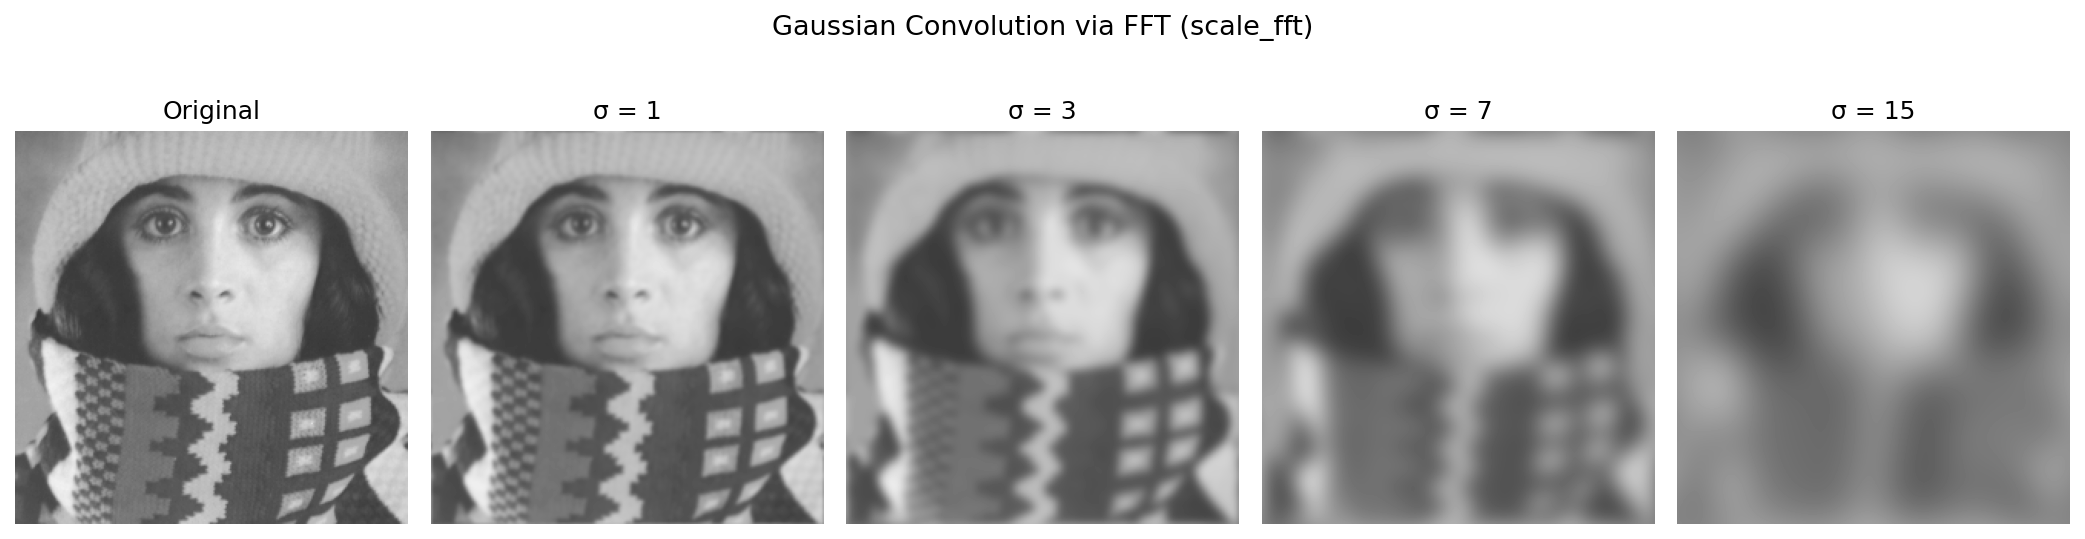
\includegraphics[width=\textwidth]{scale_fft.png}
    \caption{Gaussian smoothing of \texttt{trui.png} via \texttt{scale\_fft} at $\sigma \in \{1, 3, 7, 15\}$.}
\end{figure}

As $\sigma$ increases, $H(u,v)$ narrows in the frequency domain, suppressing progressively more high-frequency content. At $\sigma = 1$ only the finest details are smoothed; at $\sigma = 15$ edges, textures, and facial features are almost entirely removed. This illustrates the duality of the Gaussian: a wider spatial filter corresponds to a narrower frequency response acting as a low-pass filter.

\end{document}
